\chapter{Estymacja w modelu Coxa metodą stochastycznego spadku gradientu}\label{rozdz4}

Poniższy rozdział przedstawia implementację oraz zastosowanie metody stochastycznego spadku gradientu do estymacji współczynników w modelu proporcjonalnych hazardów Coxa. Jest to główny cel pracy. Poniższe rozważania odnośnie podejścia do stosowania tej metody w tym konkretnym modelu nie są oparte na żadnej literaturze ze względu na jej brak.

W czasie powstawania pracy nawiązano jedynie nieznaczną wymianę informacji z pracownikami \textit{Harvard Laboratory for Applied Statistical Methodology \& Data Science}, dzięki której dowiedziano się że podjęte zostały kroki w kierunku stworzenia podwalin pod teorię do omawianego zagadnienia, jednak ewentualne publikacje nie zostały jeszcze dokończone. Przedsmak niedokończonej implementacji algorytmu przez pracowników wyżej wymienionego laboratorium można znaleźć w \cite{sgdpkg}.

W procesie estymacji współczynników w omawianym modelu wykorzystano pochodne cząstkowe częściowej funkcji log-wiarogodności (\ref{score})
\begin{equation*}
U_k(\beta)=\dfrac{\partial\ell_k(\beta)}{\partial\beta_k}=\sum\limits_{i=1}^{K}\Big(X_{ik}-\dfrac{\sum\limits_{l\in \mathscr{R}(t_i)}^{} X_{lk} e^{X_l'\beta}}{\sum\limits_{l\in \mathscr{R}(t_i)}^{} e^{X_l'\beta}}\Big)=\sum\limits_{i=1}^{n}Y_i\Big(X_{ik}-\dfrac{\sum\limits_{l\in \mathscr{R}(t_i)}^{} X_{lk} e^{X_l'\beta}}{\sum\limits_{l\in \mathscr{R}(t_i)}^{} e^{X_l'\beta}}\Big)=\sum\limits_{i=1}^{n}U_{k_{i}}(\beta),
\end{equation*}
(dla $Y_i = 1$, gdy obserwacja nie była cenzurowana i $Y_i = 0$, gdy obserwacja była cenzurowana; $K$ to liczba zdarzeń; $n$ to liczba obserwacji) oraz wzór (\ref{sgdrownanie}), którego wersja z adekwatnymi oznaczeniami dla powyższej funkcji wygląda następująco
\begin{equation}\label{opta}
\beta_{k_{j+1}} = \beta_{k_{j}} - \alpha_{j}U_{k_{i}}(\beta_{k_{j}}),
\end{equation}
gdzie $j$ oznacza krok algorytmu, $i$ iteruje składniki $U_{k}$, $\alpha_j$ to długość $j$-tego kroku algorytmu, zaś $U_{k}$ to $k$-ta pochodna cząstkowa gradientu $U$ oraz $\beta_{k}$ to $k$-ta współrzędna estymowanego wektora współczynników $\beta$ o rozmiarze $p$, czyli $k=1,\dots,p$. 

Własna implementacja algorytmu w języku $\mathcal{R}$ znajduje się w podrozdziale (\ref{implemento}).

\section{Założenia i obserwacje}\label{zalozenia}

Skupiając się na informatycznym aspekcie algorytmu można stwierdzić, że idea stochastycznego spadku gradientu polega na losowaniu składnika optymalizowanej funkcji. Jednak ze statystycznego punktu widzenia, metoda stochastycznego spadku gradientu opiera się o losowanie indeksu obserwacji ze zbioru, z którego uczony jest algorytm, zanim postanowi się w jakikolwiek sposób przedstawić konkretną funkcję wiarogodności. Zatem w celu estymacji w oparciu o stochastyczny spadek gradientu w modelu Coxa, konstruując metodę, należy najpierw losować obserwacje a następnie dopiero wyznaczać formę optymalizowanej funkcji częściowej log-wiarogodności. 

Dla wielu modeli opierających się o funkcje wiarogodności te dwa punkty widzenia są równoważne, jednak dla modelu Coxa nie, gdyż niektóre składniki w funkcji log-wiarogodności są zależne od poprzednich obserwacji. W przypadku modelu ADALINE sformułowanego jak w \cite{ADALINE2}, opartego na minimalizowaniu funkcji kosztu w postaci błędu najmniejszych kwadratów, w \cite{bott2} podano postać funkcji straty oraz równanie algorytmu stochastycznego spadku gradientu jak poniżej
$$Q_{adaline} = \frac{1}{2}(y-w'\varPhi(x))^2, \ \ \ \varPhi(x) \in \mathbb{R}^d, y \in \{-1,1\},$$ 
$$w \leftarrow w + \alpha_k(y_k-w'\varPhi(x_t))\varPhi(x_t),$$
dla których widać, że w kolejnych krokach algorytmu $t$ wystarczy tylko jedna obserwacja $z_t=(x_t,y_t)$ aby poprawić oszacowanie parametru $w$.

W modelu proporcjonalnych hazardów Coxa jest to bardziej skomplikowane. Dla zadanej z góry funkcji hazardu, częściowa funkcja wiarogodności odpowiada prawdopodobieństwu tego, że obserwowane zdarzenia zdarzyłyby się dokładnie w tej kolejności w jakiej się pojawiły. To prawdopodobieństwo zależy od wszystkich obserwacji w zbiorze. Niemożliwe jest wyliczenie tego poprzez obliczenie wartości funkcji częściowej wiarogodności oddzielnie dla obserwacji o numerach od 1 do 5 i oddzielnie dla obserwacji od numerach 6 do 10, a następnie przemnożeniu wyników przez siebie. Z tej przyczyny niemożliwe jest losowanie czynników optymalizowanej funkcji przy użyciu metody stochastycznego spadku gradientu do estymacji współczynników w tym modelu. Alternatywnym podejściem do tego problemu mogłoby być pamiętanie wartości licznika i mianownika dla składników częściowej funkcji log-wiarogodności dla wszystkich zaobserwowanych czasów zdarzeń i poprawianie odpowiednich składników z wykorzystaniem świeżo zaobserwowanych obserwacji. Taki zabieg jest pamięciowo oszczędniejszy niż pamiętanie wszystkich obserwacji. \textbf{Możliwe jest też losowanie podzbioru obserwacji a następnie konstruowanie funkcji wiarogodności dla zaobserwowanego zredukowanego zbioru. Właśnie ta metoda zostanie opisana w dalszej części pracy.} Taki sposób wprowadzania obserwacji do estymacji można wykorzystać w sytuacjach, gdy mamy do czynienia z nieskończonym napływem nowych obserwacji a interesują nas oszacowania estymowanych parametrów modelu $\beta_k, k=1,\dots,p$ dla obecnie zaobserwowanych i wykorzystanych obserwacji. Proces ten ma dwie zalety: nie dość, że dla nowych obserwacji model jest w stanie na bazie obecnych oszacowań parametrów dokonać predykcji proporcji hazardów, to dodatkowo po każdej porcji obserwacji aktualizuje parametry modelu.

Ponieważ
omawiane algorytmy rozwiązują problem minimalizacji badanej funkcji, zaś
celem estymacji w modelu Coxa jest znalezienie parametrów modelu
maksymalizujących funkcję częściowej log-wiarogodności, zatem wzięcie do
minimalizacji funkcji z przeciwnym znakiem doprowadzi do wykorzystania
metod znajdujących minimum do znalezienia maksimum. 

Zakładając,~że dla~\(j\)-ego kroku
algorytmu i \(k\)-tej pochodnej cząstkowej dysponuje się zaobserwowanym podzbiorem
\(\mathcal{B}\), częściową funkcję wiarogodności dla zaobserwowanego podzbioru obserwacji \(\mathcal{B}\) wykorzystywaną do minimalizacji można zapisać następująco
\begin{equation}
-U^\mathcal{B}_k(\beta_j)=-\sum\limits_{i \in \mathcal{B}_\text{ind}}^{}U^\mathcal{B}_{k_{i}}(\beta_j)=-\sum\limits_{i \in \mathcal{B}_\text{ind}}^{}Y_i\Big(X_{ik}-\dfrac{\sum\limits_{l\in \mathscr{R}_\mathcal{B}(t_i)}^{} X_{lk} e^{X_l'\beta_j}}{\sum\limits_{l\in \mathscr{R}_\mathcal{B}(t_i)}^{} e^{X_l'\beta_j}}\Big),
\end{equation}
gdzie indeksy obserwacji należące do zbioru \(\mathcal{B}\) definiuje się jako
\(\mathcal{B}_{\text{ind}} = \{i: X_i \in \mathcal{B} \}\), zaś
\(\mathscr{R}_\mathcal{B}(t_i)\) to zbiór ryzyka dla podzbioru
\(\mathcal{B}\) w czasie \(t_i\).

Postać powyższej funkcji nasuwa pewne obserwacje. Dla danego kroku algorytmu, obecnie wykorzystywany zaobserwowany podzbiór obserwacji \(\mathcal{B}\)
\begin{itemize}
\item \textit{nie powinien składać się jedynie z obserwacji cenzurowanych}. \newline \ \newline Dla podzbioru zawierającego jedynie takie obserwacje wartość pochodnej cząstkowej funkcji log-wiarogodności jest równa zero, ze względu na czynniki $Y_i$, które dla obserwacji cenzurowanych są równe zero. Zerowa wartość pochodnej cząstkowej funkcji log-wiarogodności doprowadzi do niezmienienia się optymalizowanych parametrów we wzorze (\ref{opta}), a co za tym idzie, doprowadzi do przerwania optymalizacji.
\item \textit{nie powinien składać się jedynie z jednej obserwacji}. \newline \ \newline  
W takim przypadku wartość pochodnej cząstkowej funkcji log-wiarogodności jest również równa zero, bez względu na to czy obserwacja była cenzurowana czy nie. Zerowa wartość pochodnej cząstkowej funkcji log-wiarogodności doprowadzi do niezmienienia się optymalizowanych parametrów we wzorze (\ref{opta}), a co za tym idzie, doprowadzi do przerwania optymalizacji.
\item \textit{nie powinien zawierać tylko jednej obserwacji niecenzurowanej w zbiorze, która dodatkowo ma największy czas bycia pod obserwacją}. \newline \ \newline 
W tej sytuacji jedyny niezerowy czynnik w całej pochodnej cząstkowej funkcji log-wiarogodności zajdzie tylko dla obserwacji niecenzurowanej, dla której zbiór ryzyka będzie zawierał tylko nią, co da ostatecznie zerową wartość pochodnej cząstkowej optymalizowanej funkcji log-wiarogodności, co doprowadzi do przerwania optymalizacji.
\end{itemize}

Dodatkowo nie dochodzi do wykorzystania obserwacji cenzurowanych, gdy:
\begin{itemize}
\item \textit{zaobserwowany zbiór zawiera obserwacje cenzurowane, które wszystkie mają czasy obserwacji krótsze niż najmniejszy czas obserwacji dla obserwacji niecenzurowanej}. \newline \ \newline 
Obserwacje cenzurowane niosą ze sobą mniej informacji, jednak teoria analizy przeżycia stara się je maksymalnie wykorzystać, stąd uwzględnia się ich udział w zbiorze ryzyka przy estymacji fragmentów funkcji log-wiarogodności dla obserwacji niecenzurowanych. W sytuacji, gdy wszystkie obserwacje cenzurowane mają czas obserwacji krótszy niż najmniejszy czas obserwacji dla obserwacji niecenzurowanej w podzbiorze, nie dochodzi do wykorzystania obserwacji cenzurowanych w jakikolwiek sposób przy estymacji współczynników w danym kroku algorytmu.
\end{itemize}

Mając na względzie te uwagi, w sytuacji gdy zaobserwuje się podzbiór, który spełnia jeden z wyżej wymienionych warunków, można zamiast wykorzystywać ten zbiór do estymacji można go dołączyć do kolejnego podzbioru, który ma być zaobserwowany.

\newpage
\section{Implementacja}\label{implemento}

Omówiona w tym rozdziale metoda estymacji metodą stochastycznego spadku gradientu dla modelu proporcjonalnych hazardów Coxa została zaimplementowana w języku $\mathcal{R}$ \cite{programikr} i jest dostępna w specjalnie przygotowanym pakiecie o nazwie \texttt{coxphSGD()}, który można pobrać z internetu i zainstalować poleceniem
\begin{Shaded}
\begin{Highlighting}[]
\NormalTok{devtools::}\KeywordTok{install_github}\NormalTok{(}\StringTok{"MarcinKosinski/coxphSGD"}\NormalTok{)}
\end{Highlighting}
\end{Shaded}

Dokumentacja wraz z opisem argumentów w języku angielskim funkcji \texttt{coxphSGD()}, która estymuje współczynniki w modelu
proporcjonalnych hazardów Coxa metodą stochastycznego spadku gradientu, dostępna jest w Dodatku \ref{docCoxSGD}.
Starano zachować jednorodność kolejności i nazewnictwa parametrów z funkcją \texttt{coxph()} z pakietu \texttt{survival} \cite{ther}, \cite{survival}.

Implementacja algorytmu estymacji w modelu Coxa metodą stochastycznego spadku gradientu opiera się na poniższym pseudo-kodzie i zakłada, że kolejne podzbiory \(\mathcal{B}\) dostarczane są jako kolejne elementy listy.
\subsubsection{Estymacja~w~modelu~Coxa~metodą~stochastycznego~spadku~gradientu}


\begin{Shaded}
\begin{Highlighting}[]
                    \CommentTok{# wstępna inicjalizacja parametrów}
\NormalTok{eps =}\StringTok{ }\FloatTok{1e-5}                               \CommentTok{# warunek stopu.}

\NormalTok{n =}\StringTok{ }\KeywordTok{length}\NormalTok{(data)                         }\CommentTok{# data jest listą ramek danych.}

\NormalTok{diff =}\StringTok{ }\NormalTok{eps +}\StringTok{ }\DecValTok{1}                           \CommentTok{# różnice w oszacowaniach parametrów}
                                         \CommentTok{# między kolejnymi krokami.}

\NormalTok{learningRates =}\StringTok{ }\NormalTok{function(x) }\DecValTok{1}\NormalTok{/x          }\CommentTok{# długości kroku algorytmu.}

\NormalTok{beta_old =}\StringTok{ }\KeywordTok{numeric}\NormalTok{(}\DecValTok{0}\NormalTok{, }\DataTypeTok{length =} \NormalTok{k)        }\CommentTok{# punkt startowy dlugosci k,}
                                         \CommentTok{# gdzie k to liczba zmiennych}
                                         \CommentTok{# objaśniających w modelu.}

\NormalTok{max.iter =}\StringTok{ }\DecValTok{500}                           \CommentTok{# maksymalna liczba kroków.}

                              \CommentTok{# estymacja}
\NormalTok{i =}\StringTok{ }\DecValTok{1}                                    \CommentTok{# iterator kroku algorytmu.}
\NormalTok{while(i <=}\StringTok{ }\NormalTok{max.iter |}\StringTok{ }\NormalTok{diff <}\StringTok{ }\NormalTok{eps) do     }
  \NormalTok{iter =}\StringTok{ }\KeywordTok{ifelse}\NormalTok{(i mod n ==}\StringTok{ }\DecValTok{0}\NormalTok{, n, i mod n)}\CommentTok{# wybierz kolejny podzbiór batch.}
  \NormalTok{batch =}\StringTok{ }\NormalTok{data[[iter]] }
  \NormalTok{beta_new =}\StringTok{ }\NormalTok{beta_old -}\StringTok{ }\KeywordTok{learningRates}\NormalTok{(i) *}\StringTok{ }\KeywordTok{U_Batch}\NormalTok{(batch) }
                                         \CommentTok{# U_Batch to częściowa funkcja}
                                         \CommentTok{# log-wiarogdności dla zaobserwowanego}
                                         \CommentTok{# zbioru `batch`}
  \NormalTok{diff =}\StringTok{ }\KeywordTok{euclidean_dist}\NormalTok{(beta_new, beta_old) }\CommentTok{# odległość euklidesowa}
  \NormalTok{beta_old =}\StringTok{ }\NormalTok{beta_new }
  \NormalTok{i =}\StringTok{ }\NormalTok{i +}\StringTok{ }\DecValTok{1}
\NormalTok{end while}
\NormalTok{return beta_new}
\end{Highlighting}
\end{Shaded}

\textbf{Docelowa implementacja w języku $\mathcal{R}$ znajduje się poniżej.}

\begin{Shaded}
\begin{Highlighting}[]
\NormalTok{coxphSGD <-}\StringTok{ }\NormalTok{function(formula, data, }\DataTypeTok{learningRates =} \NormalTok{function(x)\{}\DecValTok{1}\NormalTok{/x\},}
                    \DataTypeTok{beta_0 =} \DecValTok{0}\NormalTok{, }\DataTypeTok{epsilon =} \FloatTok{1e-5}\NormalTok{, }\DataTypeTok{max.iter =} \DecValTok{500} \NormalTok{) \{}
  \KeywordTok{checkArguments}\NormalTok{(formula, data, learningRates,}
                  \NormalTok{beta_0, epsilon) ->}\StringTok{ }\NormalTok{beta_start }\CommentTok{# check arguments}
  \NormalTok{n <-}\StringTok{ }\KeywordTok{length}\NormalTok{(data)}
  \NormalTok{diff <-}\StringTok{ }\NormalTok{epsilon +}\StringTok{ }\DecValTok{1}
  \NormalTok{i <-}\StringTok{ }\DecValTok{1}
  \NormalTok{beta_new <-}\StringTok{ }\KeywordTok{list}\NormalTok{()     }\CommentTok{# steps are saved in a list so that they can}
  \NormalTok{beta_old <-}\StringTok{ }\NormalTok{beta_start }\CommentTok{# be tracked in the future}
  \CommentTok{# estimate}
  \NormalTok{while(i <=}\StringTok{ }\NormalTok{max.iter &}\StringTok{ }\NormalTok{diff >}\StringTok{ }\NormalTok{epsilon) \{}
    \NormalTok{beta_new[[i]] <-}\StringTok{ }\KeywordTok{coxphSGD_batch}\NormalTok{(}\DataTypeTok{formula =} \NormalTok{formula, }\DataTypeTok{beta =} \NormalTok{beta_old,}
        \DataTypeTok{learningRate =} \KeywordTok{learningRates}\NormalTok{(i), }\DataTypeTok{data =} \NormalTok{data[[}\KeywordTok{ifelse}\NormalTok{(i%%n==}\DecValTok{0}\NormalTok{,n,i%%n)]])}
    \NormalTok{diff <-}\StringTok{ }\KeywordTok{sqrt}\NormalTok{(}\KeywordTok{sum}\NormalTok{((beta_new[[i]] -}\StringTok{ }\NormalTok{beta_old)^}\DecValTok{2}\NormalTok{))}
    \NormalTok{beta_old <-}\StringTok{ }\NormalTok{beta_new[[i]]}
    \NormalTok{i <-}\StringTok{ }\NormalTok{i +}\StringTok{ }\DecValTok{1}  
  \NormalTok{\}}
  \CommentTok{# return results}
  \KeywordTok{list}\NormalTok{(}\DataTypeTok{Call =} \KeywordTok{match.call}\NormalTok{(), }\DataTypeTok{epsilon =} \NormalTok{epsilon, }\DataTypeTok{learningRates =} \NormalTok{learningRates,}
       \DataTypeTok{steps =} \NormalTok{i, }\DataTypeTok{coefficients =} \KeywordTok{c}\NormalTok{(}\KeywordTok{list}\NormalTok{(beta_start), beta_new))}
\NormalTok{\}}

\NormalTok{coxphSGD_batch <-}\StringTok{ }\NormalTok{function(formula, data, learningRate, beta)\{}
  \CommentTok{# collect times, status, variables and reorder samples }
  \CommentTok{# to make the algorithm more clear to read and track}
  \NormalTok{batchData <-}\StringTok{ }\KeywordTok{prepareBatch}\NormalTok{(}\DataTypeTok{formula =} \NormalTok{formula, }\DataTypeTok{data =} \NormalTok{data)}
  \CommentTok{# calculate the log-likelihood for this batch sample}
  \NormalTok{partial_sum <-}\StringTok{ }\KeywordTok{list}\NormalTok{()}
  \NormalTok{for(k in }\DecValTok{1}\NormalTok{:}\KeywordTok{nrow}\NormalTok{(batchData)) \{}
    \CommentTok{# risk set for current time/observation}
    \NormalTok{risk_set <-}\StringTok{ }\NormalTok{batchData %>%}\StringTok{ }\KeywordTok{filter}\NormalTok{(times >=}\StringTok{ }\NormalTok{batchData$times[k])}
    
    \NormalTok{nominator <-}\StringTok{ }\KeywordTok{apply}\NormalTok{(risk_set[, -}\KeywordTok{c}\NormalTok{(}\DecValTok{1}\NormalTok{,}\DecValTok{2}\NormalTok{)], }\DataTypeTok{MARGIN =} \DecValTok{1}\NormalTok{, function(element)\{}
      \NormalTok{element *}\StringTok{ }\KeywordTok{exp}\NormalTok{(element *}\StringTok{ }\NormalTok{beta)}
    \NormalTok{\}) %>%}\StringTok{ }\KeywordTok{rowSums}\NormalTok{()}
      
    \NormalTok{denominator <-}\StringTok{ }\KeywordTok{apply}\NormalTok{(risk_set[, -}\KeywordTok{c}\NormalTok{(}\DecValTok{1}\NormalTok{,}\DecValTok{2}\NormalTok{)], }\DataTypeTok{MARGIN =} \DecValTok{1}\NormalTok{, function(element)\{}
      \KeywordTok{exp}\NormalTok{(element *}\StringTok{ }\NormalTok{beta)}
    \NormalTok{\}) %>%}\StringTok{ }\KeywordTok{rowSums}\NormalTok{()}
      
    \NormalTok{partial_sum[[k]] <-}\StringTok{ }
\StringTok{      }\NormalTok{batchData[k, }\StringTok{"event"}\NormalTok{] *}\StringTok{ }\NormalTok{(batchData[k, -}\KeywordTok{c}\NormalTok{(}\DecValTok{1}\NormalTok{,}\DecValTok{2}\NormalTok{)] -}\StringTok{ }\NormalTok{nominator/denominator)}
  \NormalTok{\}}
  \KeywordTok{do.call}\NormalTok{(rbind, partial_sum) %>%}
\StringTok{    }\KeywordTok{colSums}\NormalTok{() ->}\StringTok{ }\NormalTok{U_batch}
  
  \KeywordTok{return}\NormalTok{(beta +}\StringTok{ }\NormalTok{learningRate *}\StringTok{ }\NormalTok{U_batch)}
\NormalTok{\}}
\end{Highlighting}
\end{Shaded}
\newpage
\section{Symulacje estymacji w modelu Coxa}

Dzięki przygotowanej w rozdziale \ref{symWei} funkcji \texttt{dataCox()} możliwe będzie symulacyjne zbadanie zachowania się współczynników w modelu Coxa w trakcie estymacji metodą stochastycznego spadku gradientu, której algorytm został zaimplementowany w rozdziale \ref{implemento}. Poniższe wywołanie zwraca ramkę danych o 10 tysiącach wierszy, wraz z ze sztucznie wygenerowanymi czasami z rozkładu Weibulla o parametrach $\lambda =3$ oraz $\rho =2$. Czasy cenzurowania generowane są z rozkładu wykładniczego o parametrze $5$ a ostateczne czasy bycia pod obserwacją odpowiadają współczynnikom modelu $\beta = (1,3)$. Porównując czas życia oraz czas cenzurowania wylosowany dla obserwacji, rezultacie otrzymać można czasy przeżycia oraz status zdarzenia bądź cenzurowania. 
\begin{Shaded}
\begin{Highlighting}[]
\NormalTok{x <-}\StringTok{ }\KeywordTok{matrix}\NormalTok{(}\KeywordTok{sample}\NormalTok{(}\DecValTok{0}\NormalTok{:}\DecValTok{1}\NormalTok{, }\DataTypeTok{size =} \DecValTok{20000}\NormalTok{, }\DataTypeTok{replace =} \OtherTok{TRUE}\NormalTok{), }\DataTypeTok{ncol =} \DecValTok{2}\NormalTok{)}
\NormalTok{dCox <-}\StringTok{ }\KeywordTok{dataCox}\NormalTok{(}\DecValTok{10}\NormalTok{^}\DecValTok{4}\NormalTok{, }\DataTypeTok{lambda =} \DecValTok{3}\NormalTok{, }\DataTypeTok{rho =} \DecValTok{2}\NormalTok{, x, }\DataTypeTok{beta =} \KeywordTok{c}\NormalTok{(}\DecValTok{1}\NormalTok{,}\DecValTok{3}\NormalTok{), }\DataTypeTok{censRate =} \DecValTok{5}\NormalTok{) }
\end{Highlighting}
\end{Shaded}
Funkcja \texttt{simulateCoxSGD()} opisana w Dodatku \ref{coxKody123} sześciokrotnie dzieli wygenerowany zbiór danych odpowiednio na 10, 30, 60, 90, 120 i 200 podzbiorów losowych długości ustawiając obserwacje w losowej kolejności, a następnie wykorzystuję funkcję \texttt{coxphSGD()} do wyznaczenia wartości współczynników w kolejnych krokach estymacji funkcji log-wiarogodności dla modelu Coxa przy pomocy metody stochastycznego spadku gradientu. Dzięki tak otrzymany współczynnikom modelu w kolejnych krokach algorytmu dla różnych podziałów zbiorów, możliwe było graficzne przedstawienie trajektorii zbieżności algorytmu w zależności od ustawionego punktu startowego, warunku stopu oraz wartości ciągu odpowiadającego długościom kroków w algorytmie. 

Implementacja umożliwia ponowne wykorzystanie wszystkich zaobserwowanych podzbiorów danych w kolejnych krokach algorytmu, jeżeli nie pozostały już do wykorzystania żadne nowe podzbiory zaś zbieżność algorytmu, poza warunkiem stopu, zależna jest także od maksymalnej liczby iteracji, która gdy jest większa od liczby zaobserwowanych podzbiorów powoduje, że w trakcie procesu optymalizacji algorytm przechodzi do nowej epoki. 

Przykładowe wywołanie funkcji \texttt{simulateCoxSGD()} znajduje się poniżej

\begin{Shaded}
\begin{Highlighting}[]
\KeywordTok{simulateCoxSGD}\NormalTok{(dCox, }\DataTypeTok{learningRates =} \NormalTok{function(x)\{}\DecValTok{1}\NormalTok{/(}\DecValTok{100}\NormalTok{*}\KeywordTok{sqrt}\NormalTok{(x))\},}
               \DataTypeTok{max.iter =} \DecValTok{10}\NormalTok{, }\DataTypeTok{epsilon =} \FloatTok{1e-5}\NormalTok{, }\DataTypeTok{beta_0 =} \KeywordTok{c}\NormalTok{(}\DecValTok{2}\NormalTok{,}\DecValTok{2}\NormalTok{))}
\end{Highlighting}
\end{Shaded}
gdzie w tym wypadku parametr \texttt{max.iter} odpowiada za liczbę epok do wykorzystania, \texttt{learningRates} to funkcja odpowiedzialna za wyznaczenie długości kolejnych kroków algorytmu, \texttt{dCox} to dane do analizy przygotowane w postaci jaką zwraca funkcja \texttt{dataCox()}, \texttt{epsilon} to warunek stopu, zaś \texttt{beta\_0} to punkt startowy algorytmu.

Na Rysunkach (\ref{rysCox}) - (\ref{rysCox4}) przedstawiono symulacje zbieżności procesu optymalizacji częściowej funkcji log-wiarogodności dla zaobserwowanego podzbioru obserwacji w modelu Coxa proporcjonalnych hazardów, z wykorzystanie algorytmu stochastycznego spadku gradientu. Trajektorie zbieżności zależne są od ustawionego punktu startowego, warunku stopu oraz wartości ciągu odpowiadającego długościom kroków w algorytmie. Dodatkowo przedstawiono warstwice częściowej funkcji log-wiarogodności wyliczone dla wszystkich zaobserwowanych podzbiorów połączonych w jeden. Trójkątem zaznaczono punkt startowy algorytmu, kwadratem zaś teoretyczne maksimum. 

\newpage
\subsubsection{Podsumowanie symulacji dla modelu proporcjonalnych hazardów Coxa}

W trakcie symulacji badano jak podział całego zbioru obserwacji na podzbiory wpływa na trajektoria optymalizacji częściowej funkcji log-wiarogodności w modelu Coxa proporcjonalnych hazardów dla zaobserwowanego podzbioru. Badano również wpływ punktu początkowego, warunku stopu, liczby epok oraz konstrukcji ciągu odpowiedzialnego za długości kroków na proces optymalizacji w tym modelu. 

Na Rysunkach (\ref{rysCox}) - (\ref{rysCox4}) zaprezentowano trajektoria dla punktów początkowych: $\beta_0 = (0,0), (2,2), (-1,4)$. Brano pod uwagę ciągi odpowiadające długościom kroków równe $\frac{1}{20\sqrt{t}}, \frac{1}{50\sqrt{t}}, \frac{1}{100\sqrt{t}}$, eksperymentowano z liczbą epok ustalaną na $1,5,10$ oraz sprawdzano jak zachowają się trajektoria dla warunków stopu $\epsilon=10^{-6}, \epsilon=10^{-5}$. Dla ciągów odpowiadającym długościom kroków ustalanym na $\frac{1}{20t}, \frac{1}{50t}, \frac{1}{100t}$ algorytm nie osiągał zbieżności i zatrzymywał się po maksymalnej liczbie iteracji w losowym punkcie.

Dla żadnej z symulacji algorytm nie zbiegł do punktu, w którym powinno być teoretyczne optimum. Może to wynikać z dużej liczby obserwacji cenzurowanych bądź z samej istoty losowości przy procesie generowania danych. Należy podkreślić, że dla różnych sprawdzanych wariantów procesu optymalizacji za każdym razem metoda zbiegała do tego samego punktu. Może być to optimum wynikające z postaci danych. Stochastyczny spadek gradientu nie wykorzystuje wszystkich obserwacji jednocześnie przez co trudniej zbiec do teoretycznego optimum. Warto zauważyć stabilność procesu optymalizacji dla ciągów odpowiadających za długość kroków w algorytmie, które ustawione zostały na mniejsze wartości $\frac{1}{50\sqrt{t}}, \frac{1}{100\sqrt{t}}$ (Rysunki (\ref{rysCox}) - (\ref{rysCox3})) - w przypadku ciągu o zbyt dużych wartościach początkowych ($\frac{1}{20\sqrt{t}}$) trajektoria algorytmu we wczesnej fazie procesu były daleki od optimum (Rysunek (\ref{rysCox4})). Dzięki ukazanym warstwicom funkcji częściowej log-wiarogodności skonstruowanym na całych danych, widać, że poczynając od punktu startowego algorytm w różnych wydaniach postępuje we właściwym kierunku zbieżności i kieruje się w okolice teoretycznego optimum. Algorytm zatrzymuje się niedaleko teoretycznego optimum, jednak patrząc na rozrzedzone zagęszczenie warstwic w okolicach teoretycznego optimum, można stwierdzić, że wartości funkcji częściowej log-wiarogodności nie różnią się już na tyle, aby proces optymalizacji mógł być kontynuowany. 

Warto podkreślić, że większa liczba epok i mniejszy warunek stopu powodują jedynie poprawienie optymalizacji dla wariantów, w których cały zbiór obserwacji był podzielony na największą liczbę obserwacji, a więc każdy krok algorytmu budowany był na najmniej licznych podzbiorach.

Proces estymacji w modelu proporcjonalnych hazardów Coxa z wykorzystaniem metody stochastycznego spadku gradientu w sytuacji napływających danych wygląda na stabilny i zbiega w okolice bliskie do teoretycznego optimum, niekiedy nawet dla tylko jednej epoki. Dla dobrze dobranych parametrów optymalizacji proces może być z powodzeniem wykorzystywany do znajdowania współczynników modelu. Kluczowym momentem mającym wpływ na powodzenie optymalizacji jest wybór ciągu odpowiedzialnego za dobór długości kroków w algorytmie, więc zaleca się symulacje badające różne ciągi oraz wybranie tego ciągu, który w większości przypadków daje stabilne, jednorodne współczynniki. 

\begin{figure}[hbt!]
  %\vspace{-10pt}
  \begin{center}
   \begin{subfigure}[h!]{0.9\textwidth}
      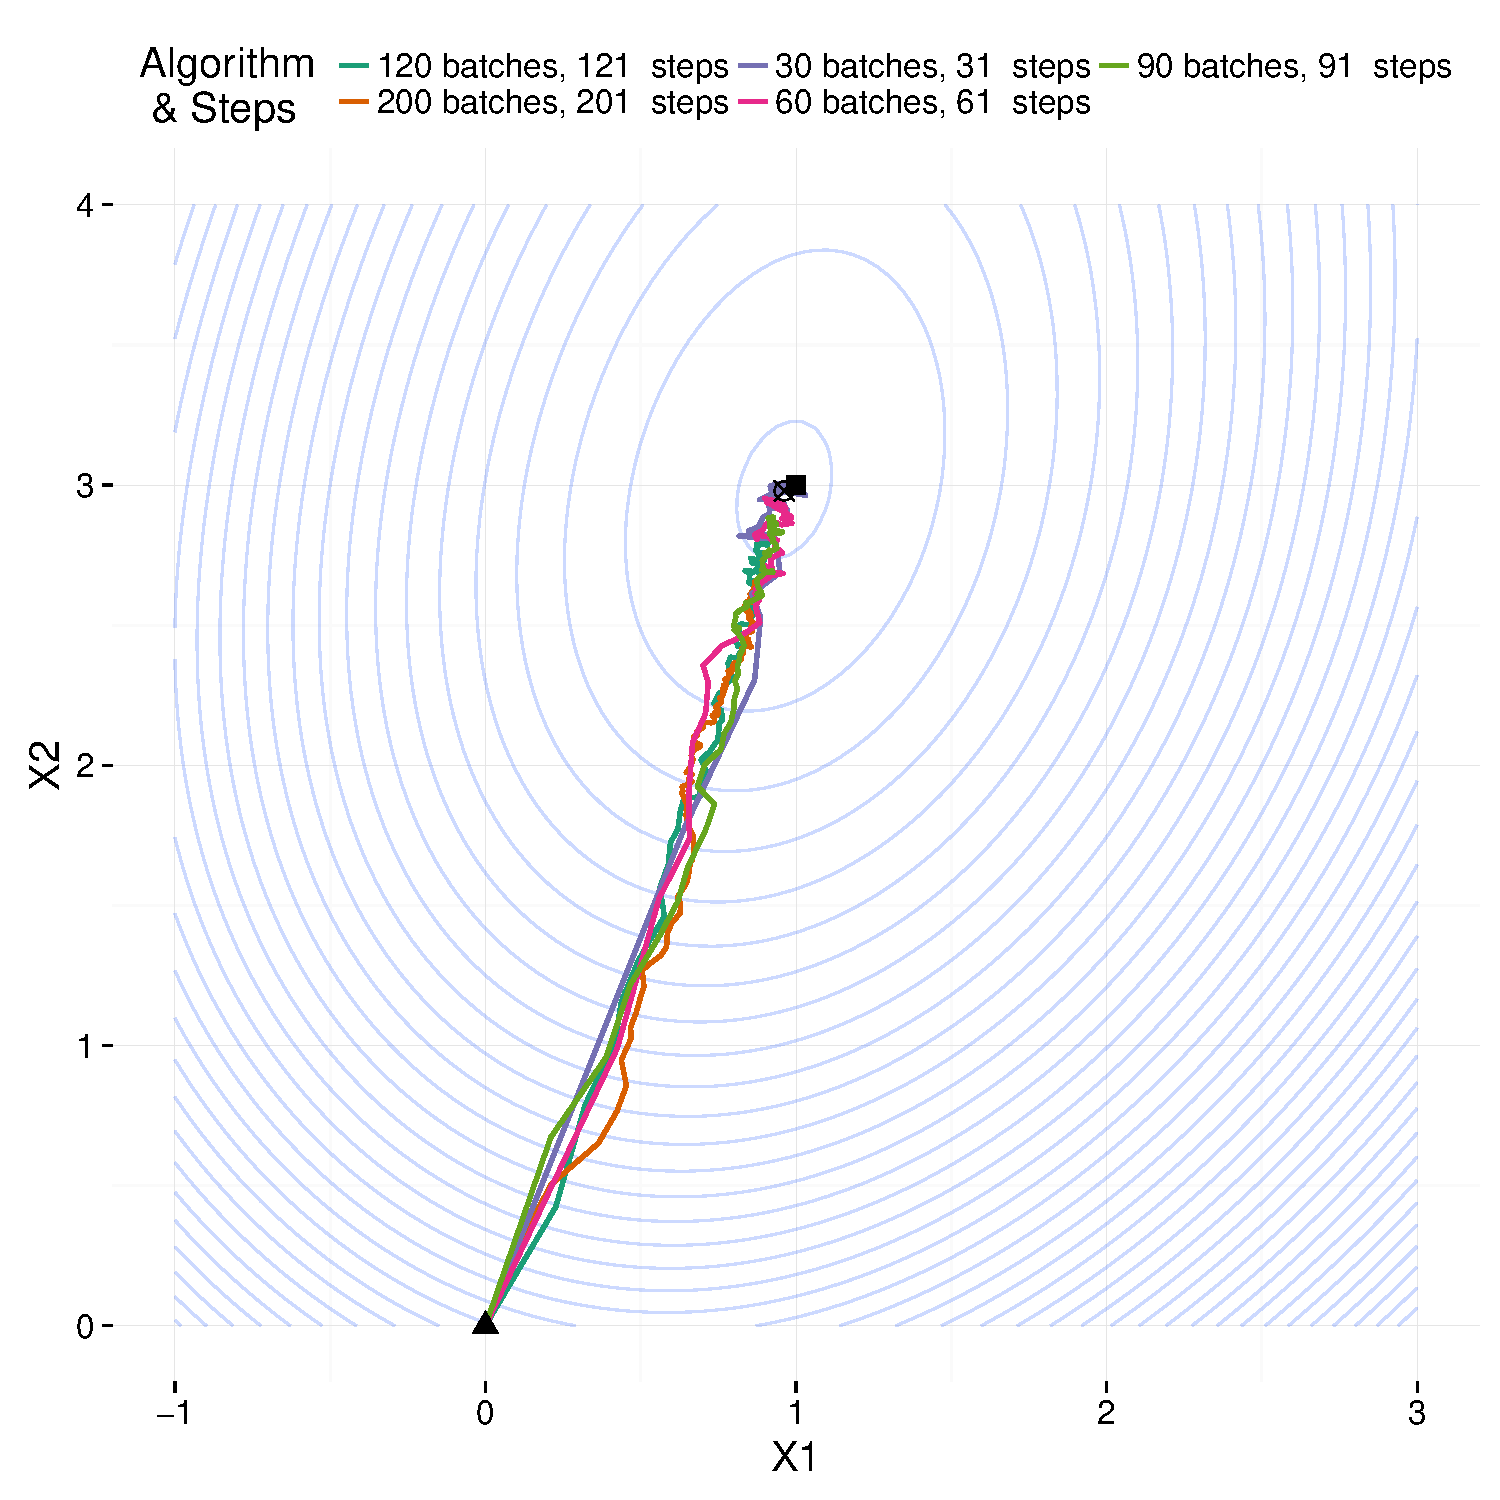
\includegraphics[width=\textwidth, height=320pt]{Obrazki/b_0_0_iter_1_e-6_50sqrt.pdf}
      \caption{$\beta_0=(0,0)$, liczba epok 1, warunek stopu: $\epsilon=10^{-6}$, długości kroków = $\frac{1}{50\sqrt{t}}$.}
   \end{subfigure}     
   \begin{subfigure}[h!]{0.9\textwidth}
      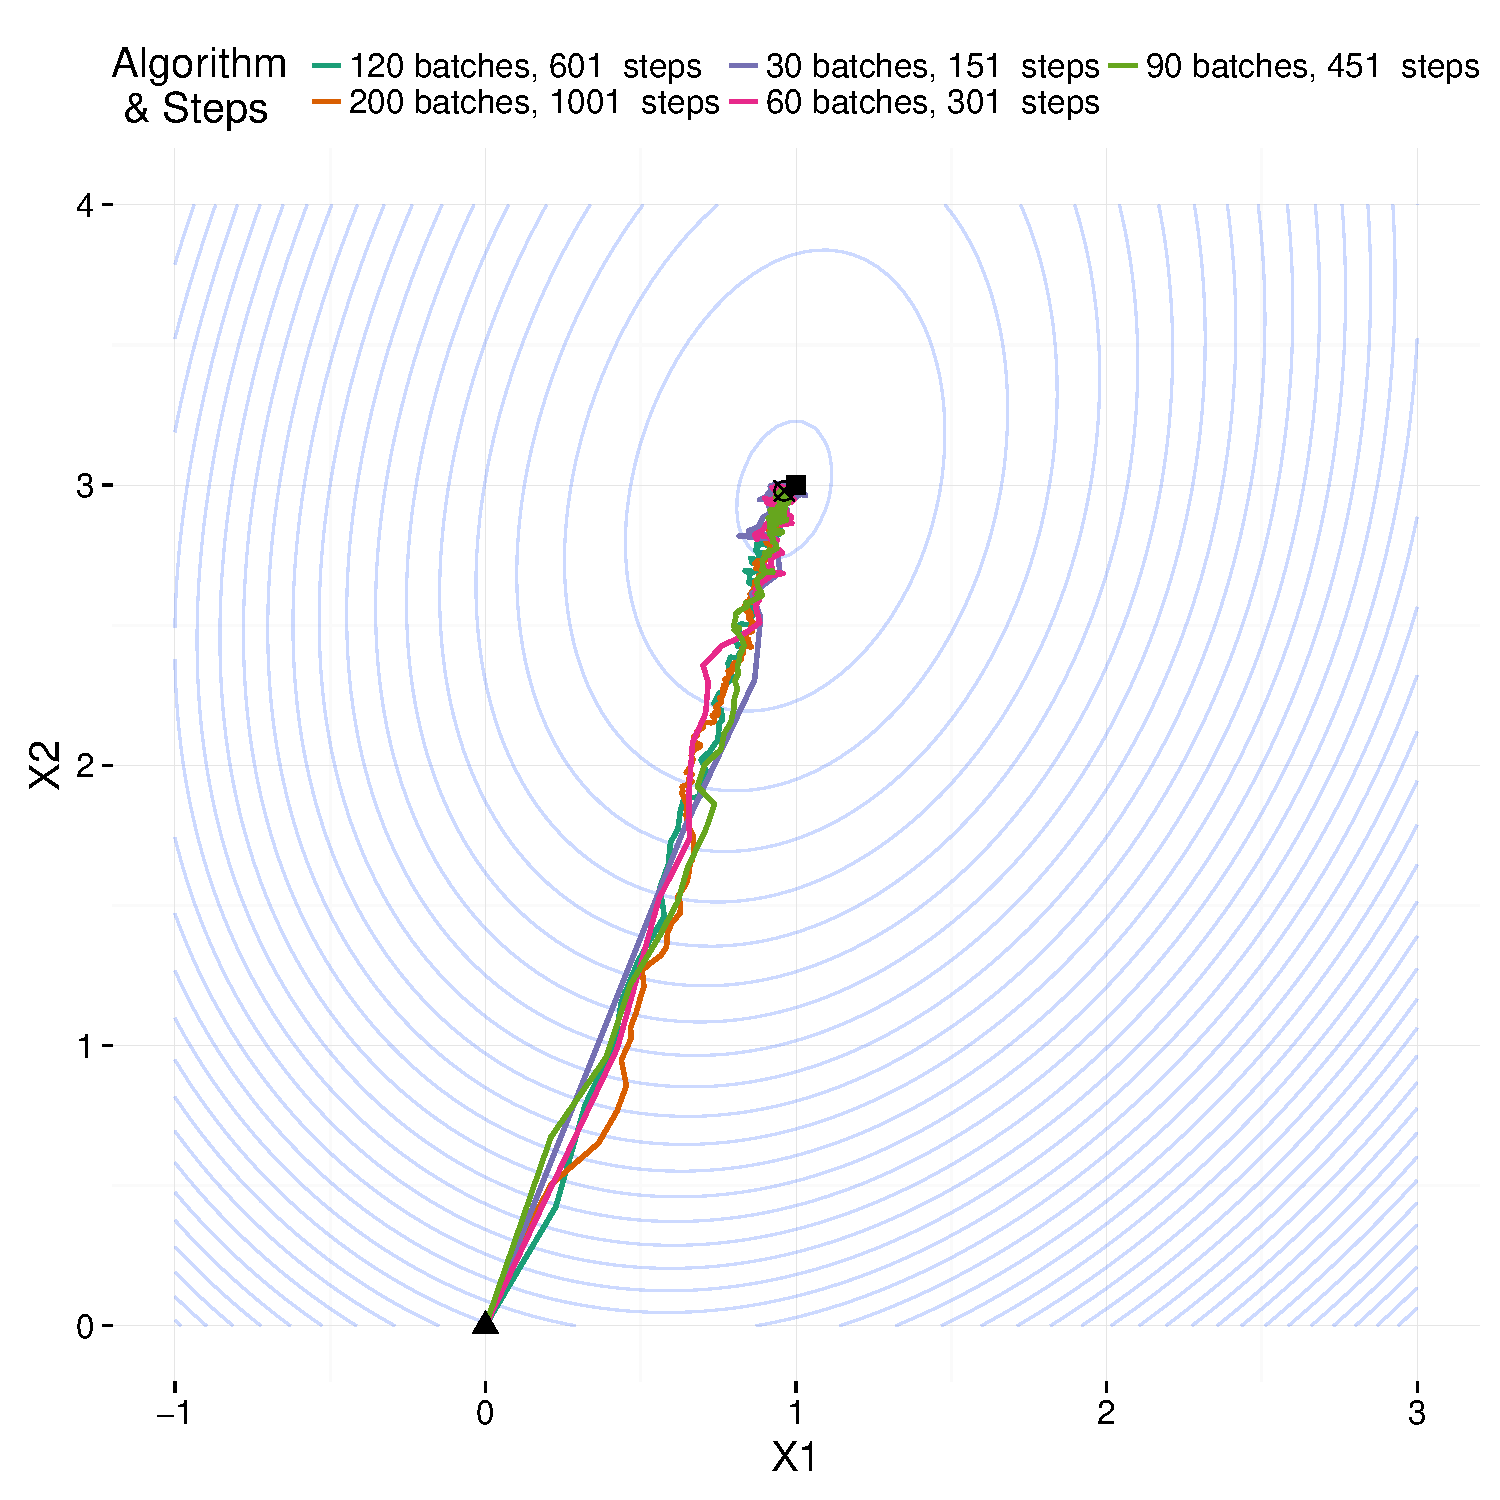
\includegraphics[width=\textwidth, height=320pt]{Obrazki/b_0_0_iter_5_e-6_50sqrt.pdf}
            \caption{$\beta_0=(0,0)$, liczba epok 5, warunek stopu: $\epsilon=10^{-6}$, długości kroków = $\frac{1}{50\sqrt{t}}$.}
   \end{subfigure}  
      \end{center}
  %\vspace{-10pt}
  \caption[Porównanie estymacji w modelu Coxa metodą stochastycznego spadku gradientu dla różnych podziałów zbioru początkowego na podzbiory.]{\label{rysCox}Porównanie estymacji w modelu Coxa metodą stochastycznego spadku gradientu dla różnych podziałów zbioru początkowego na podzbiory.}
\end{figure}



\begin{figure}[hbt!]
  %\vspace{-10pt}
  \begin{center}
   \begin{subfigure}[h!]{0.9\textwidth}
      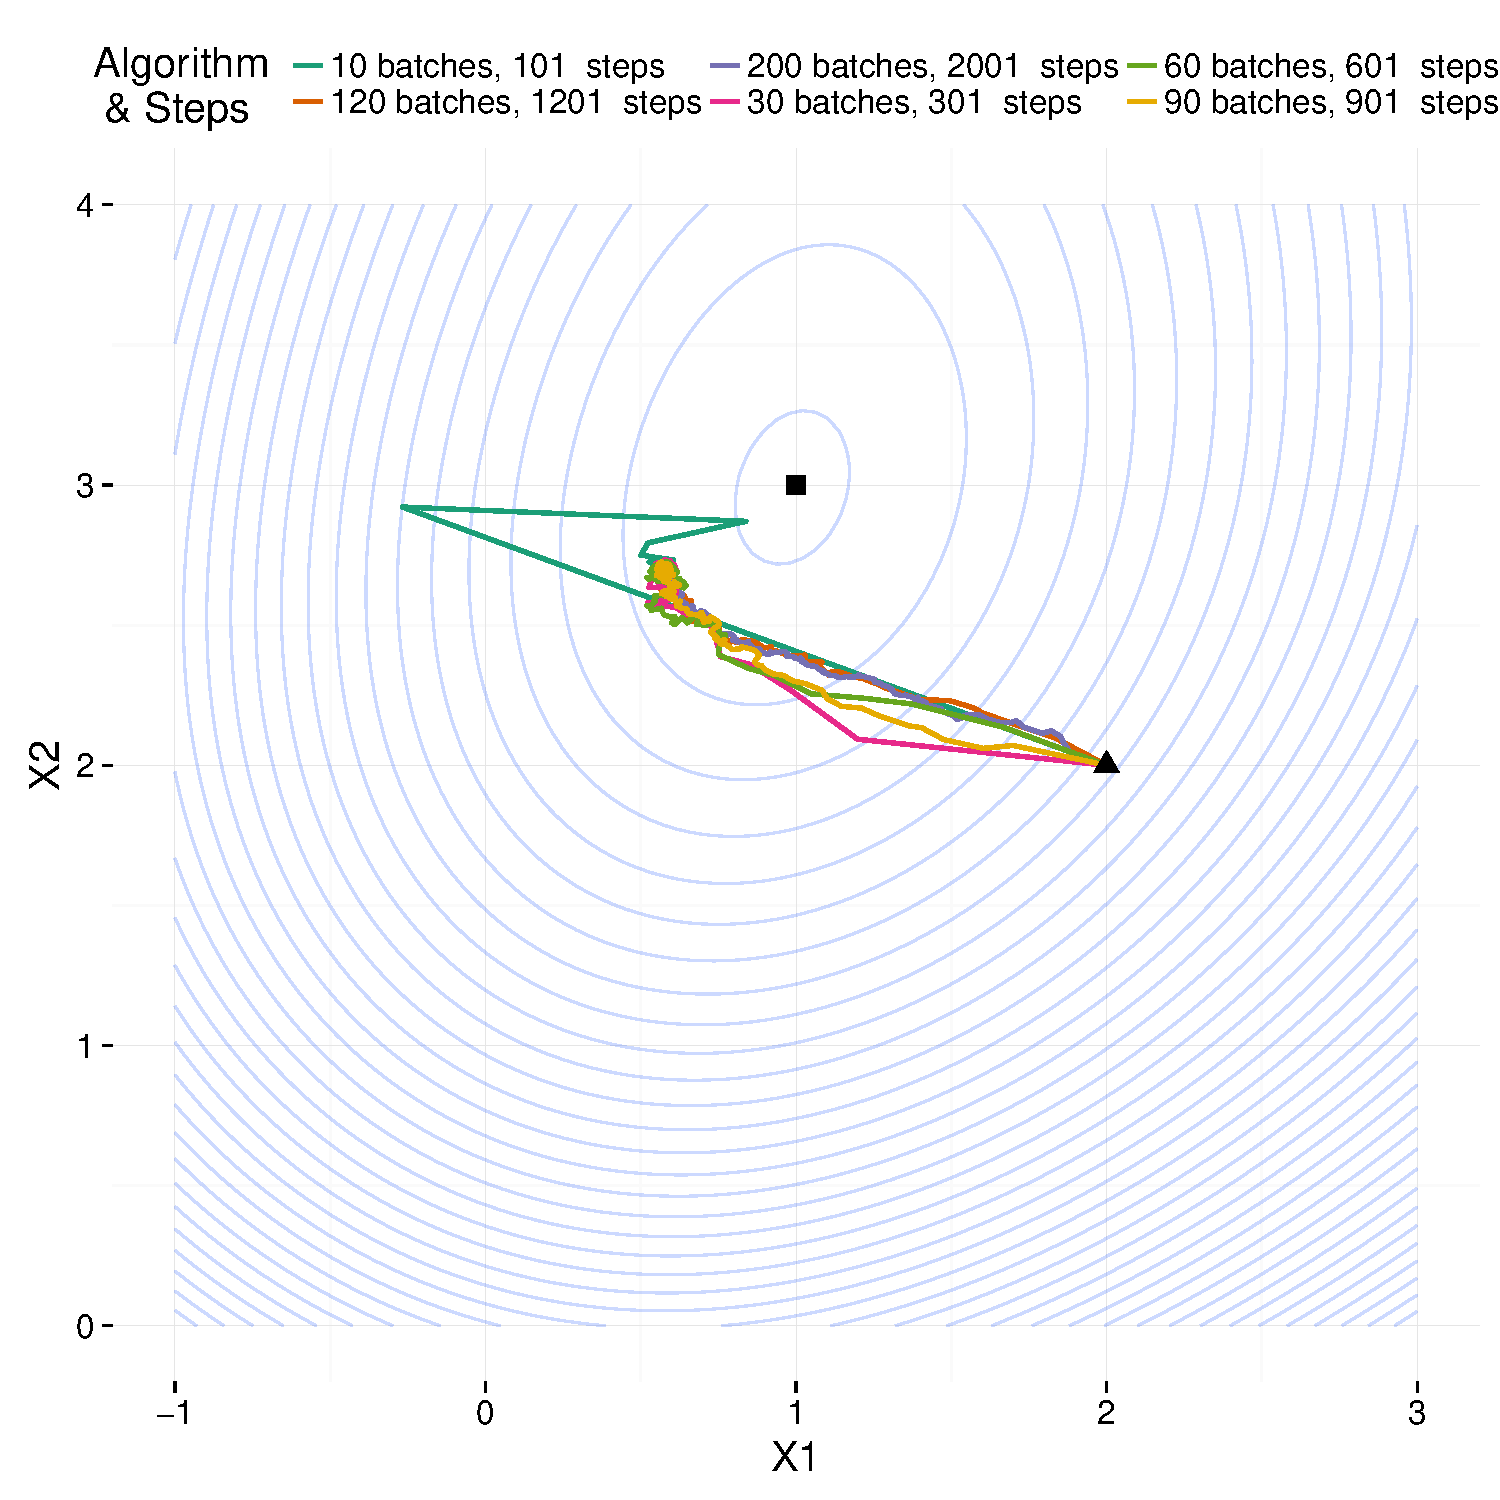
\includegraphics[width=\textwidth, height=320pt]{Obrazki/b_2_2_iter_10_e-6_50sqrt.pdf}
      \caption{$\beta_0=(2,2)$, liczba epok 10, warunek stopu: $\epsilon=10^{-6}$, długości kroków = $\frac{1}{50\sqrt{t}}$.}
   \end{subfigure}     
   \begin{subfigure}[h!]{0.9\textwidth}
      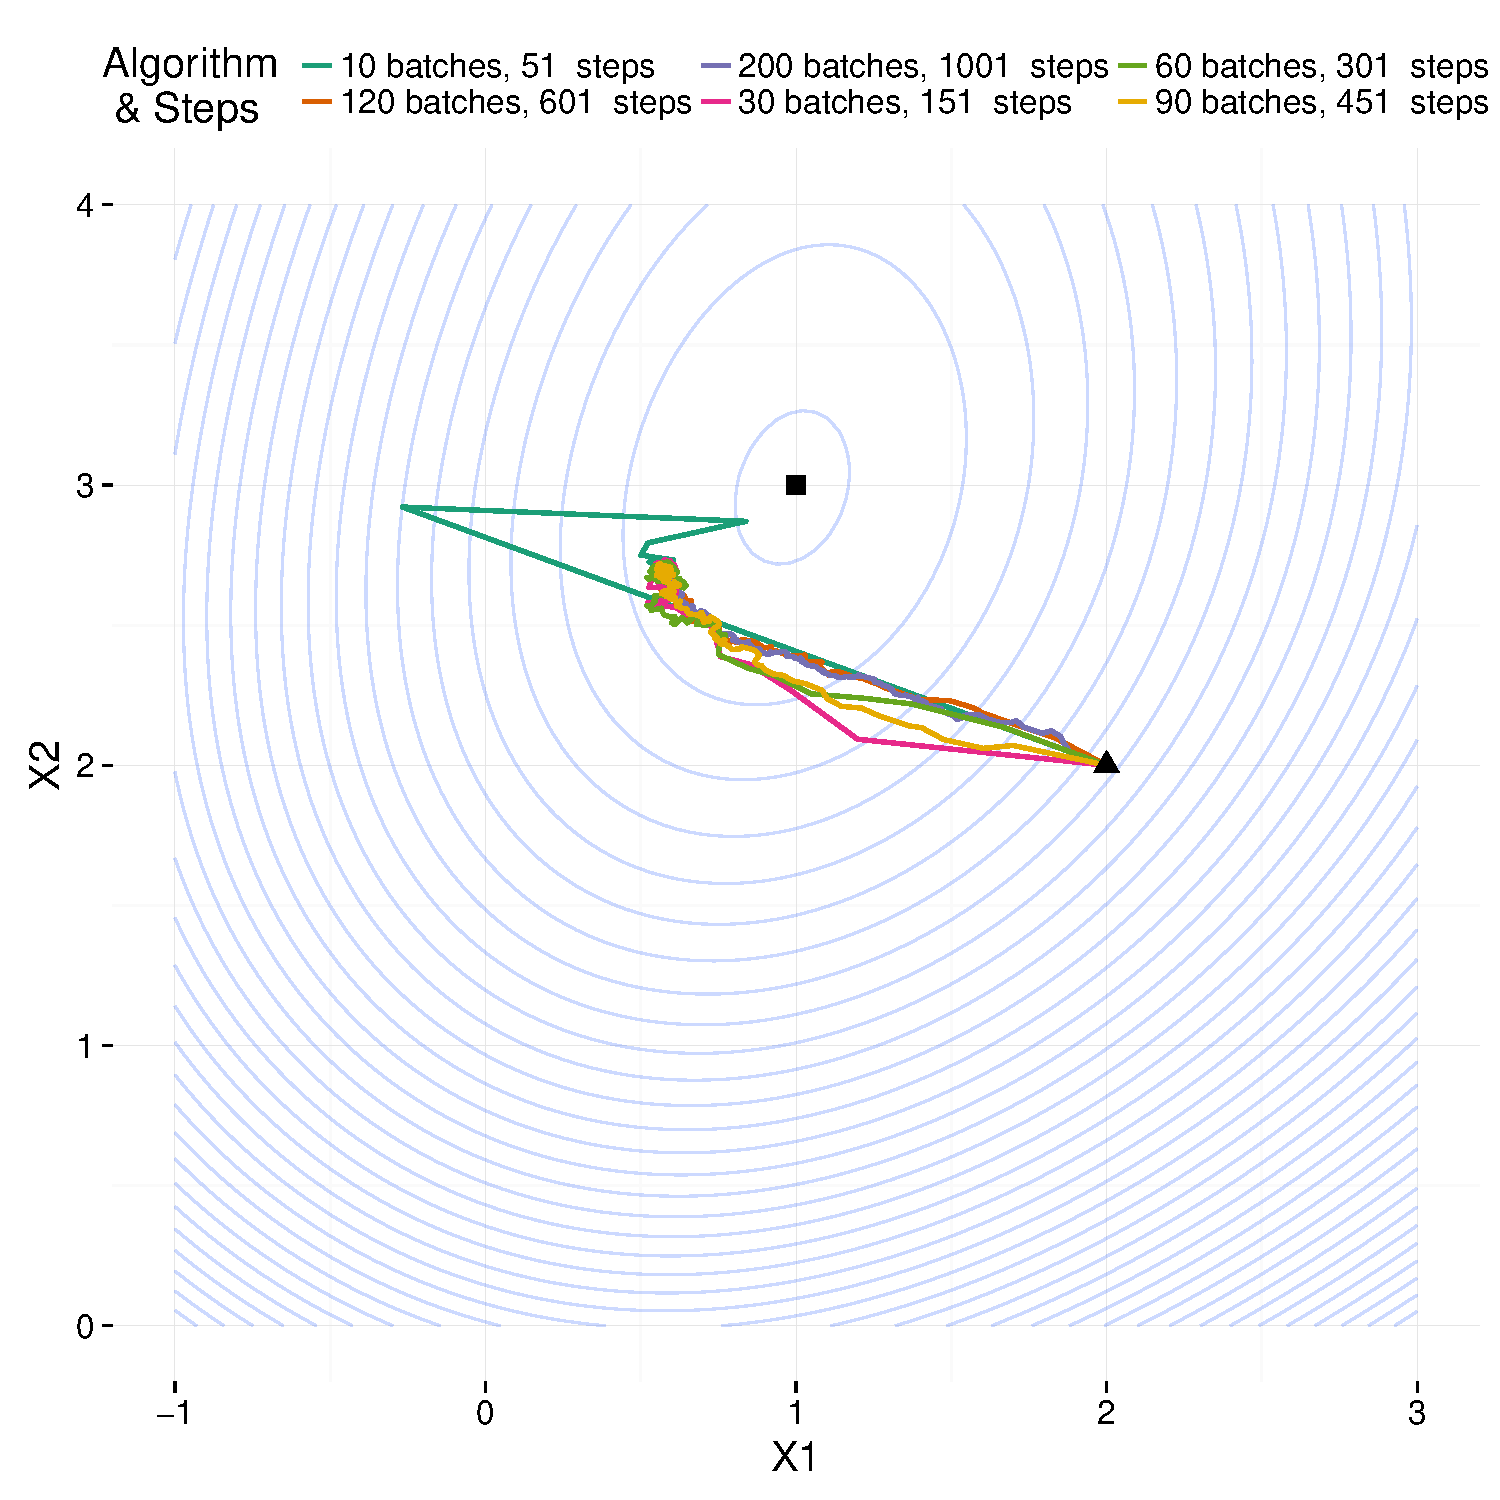
\includegraphics[width=\textwidth, height=320pt]{Obrazki/b_2_2_iter_5_e-5_50sqrt.pdf}
            \caption{$\beta_0=(2,2)$, liczba epok 5, warunek stopu: $\epsilon=10^{-5}$, długości kroków = $\frac{1}{50\sqrt{t}}$.}
   \end{subfigure}  
      \end{center}
  %\vspace{-10pt}
  \caption[Porównanie estymacji w modelu Coxa metodą stochastycznego spadku gradientu dla różnych podziałów zbioru początkowego na podzbiory.]{\label{rysCox2}Porównanie estymacji w modelu Coxa metodą stochastycznego spadku gradientu dla różnych podziałów zbioru początkowego na podzbiory.}
\end{figure}
	
	
	
	
\begin{figure}[hbt!]
  %\vspace{-10pt}
  \begin{center}
   \begin{subfigure}[h!]{0.9\textwidth}
      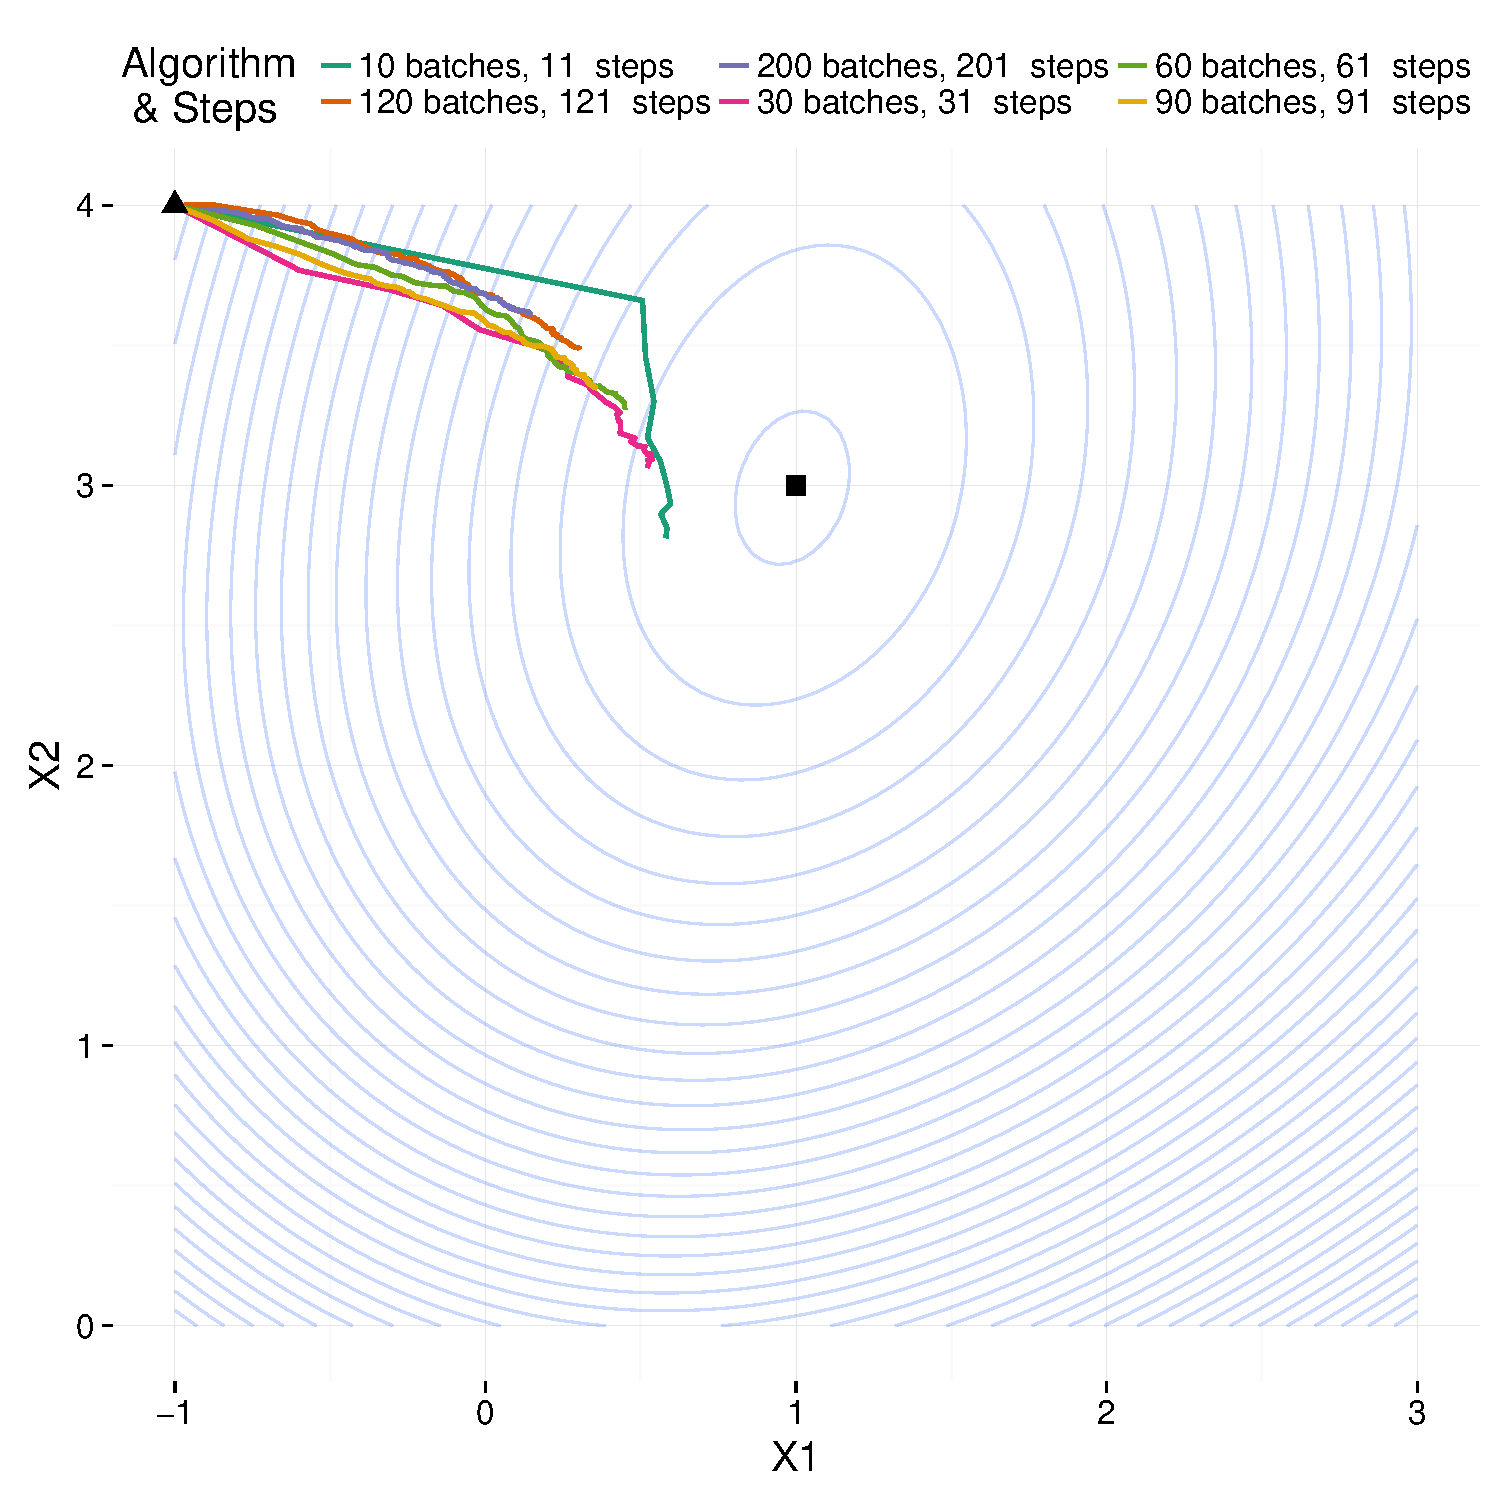
\includegraphics[width=\textwidth, height=320pt]{Obrazki/b_m1_4_iter_1_e-6_100sqrt.pdf}
      \caption{$\beta_0=(-1,4)$, liczba epok 1, warunek stopu: $\epsilon=10^{-6}$, długości kroków = $\frac{1}{100\sqrt{t}}$.}
   \end{subfigure}     
   \begin{subfigure}[h!]{0.9\textwidth}
      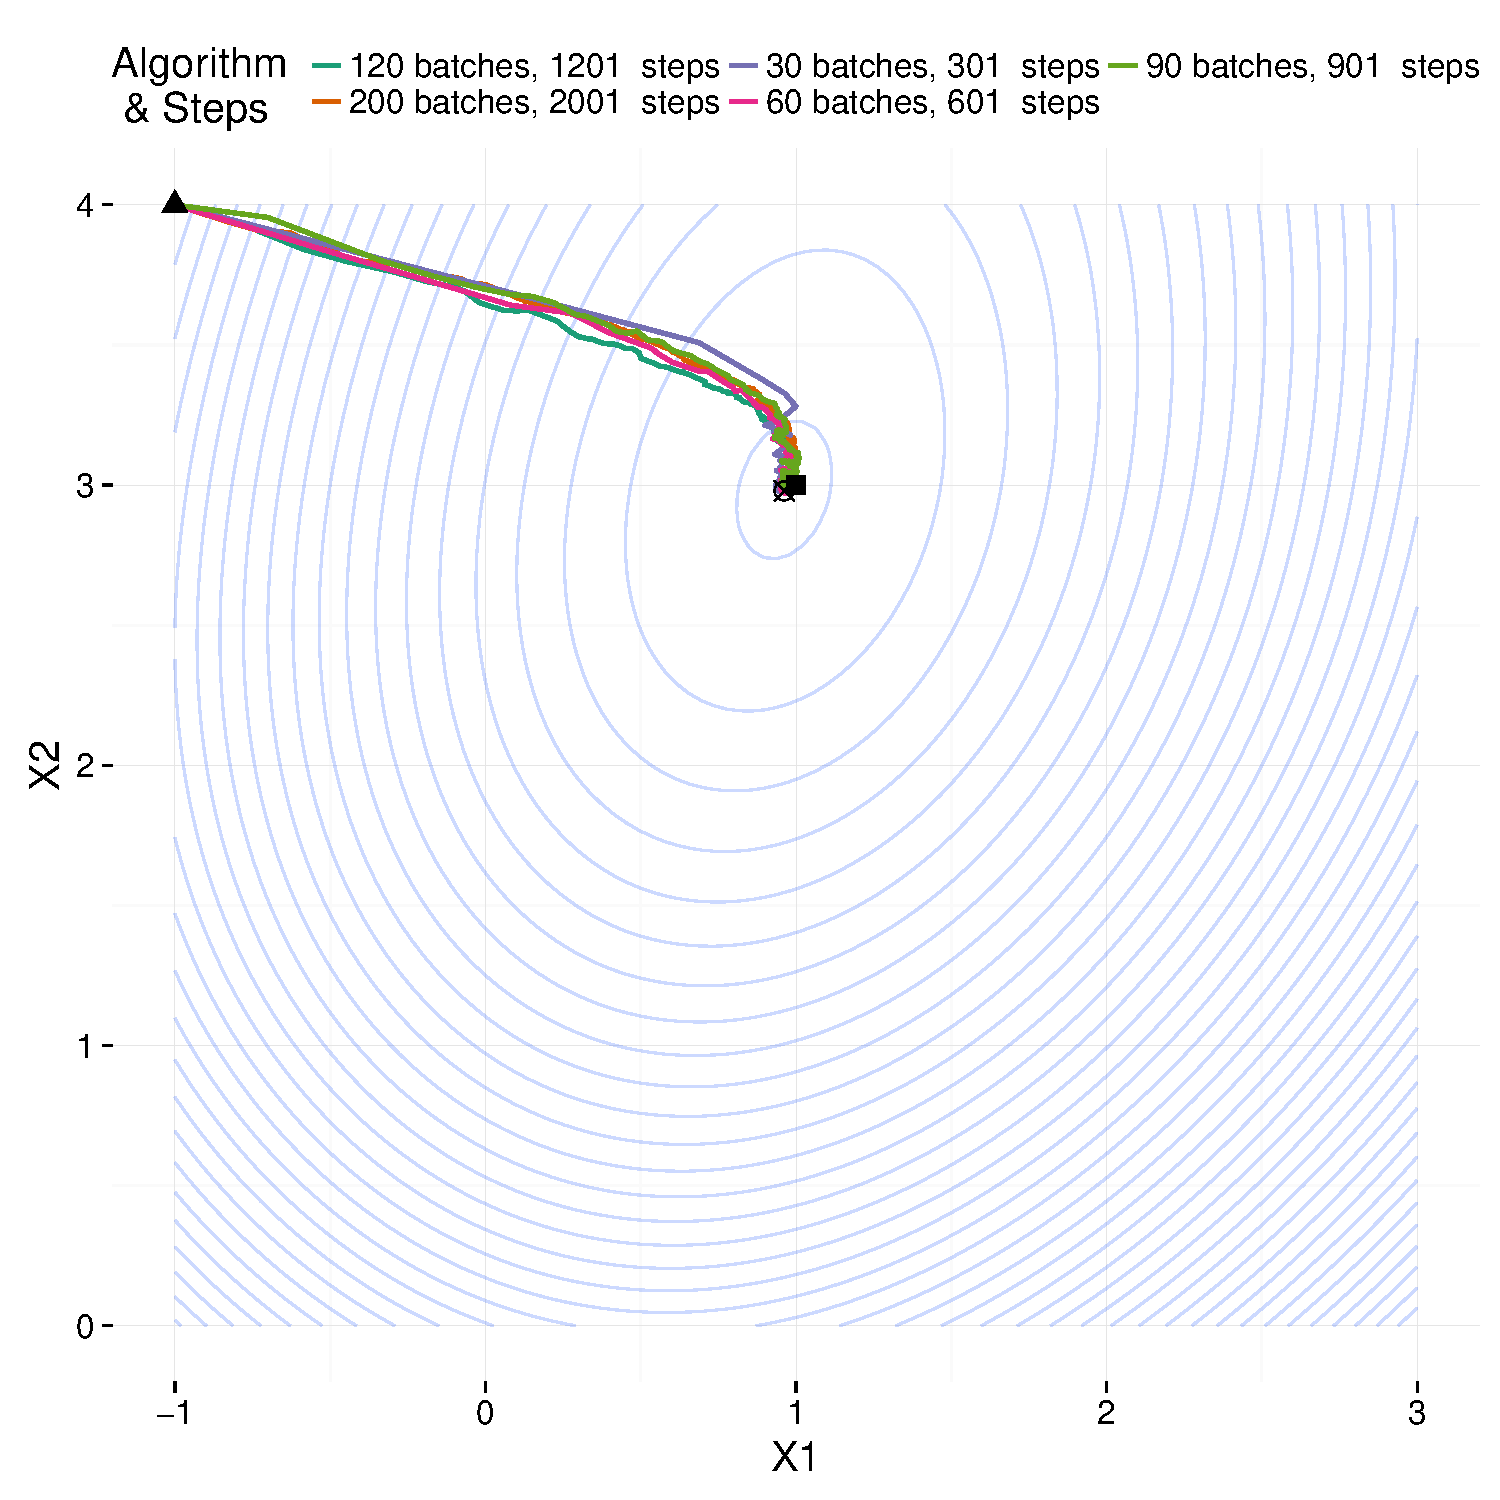
\includegraphics[width=\textwidth, height=320pt]{Obrazki/b_m1_4_iter_10_e-5_100sqrt.pdf}
            \caption{$\beta_0=(-1,4)$, liczba epok 10, warunek stopu: $\epsilon=10^{-5}$, długości kroków = $\frac{1}{100\sqrt{t}}$.}
   \end{subfigure}  
      \end{center}
  %\vspace{-10pt}
  \caption[Porównanie estymacji w modelu Coxa metodą stochastycznego spadku gradientu dla różnych podziałów zbioru początkowego na podzbiory.]{\label{rysCox3}Porównanie estymacji w modelu Coxa metodą stochastycznego spadku gradientu dla różnych podziałów zbioru początkowego na podzbiory.}
\end{figure}



\begin{figure}[hbt!]
  %\vspace{-10pt}
  \begin{center}
   \begin{subfigure}[h!]{0.9\textwidth}
      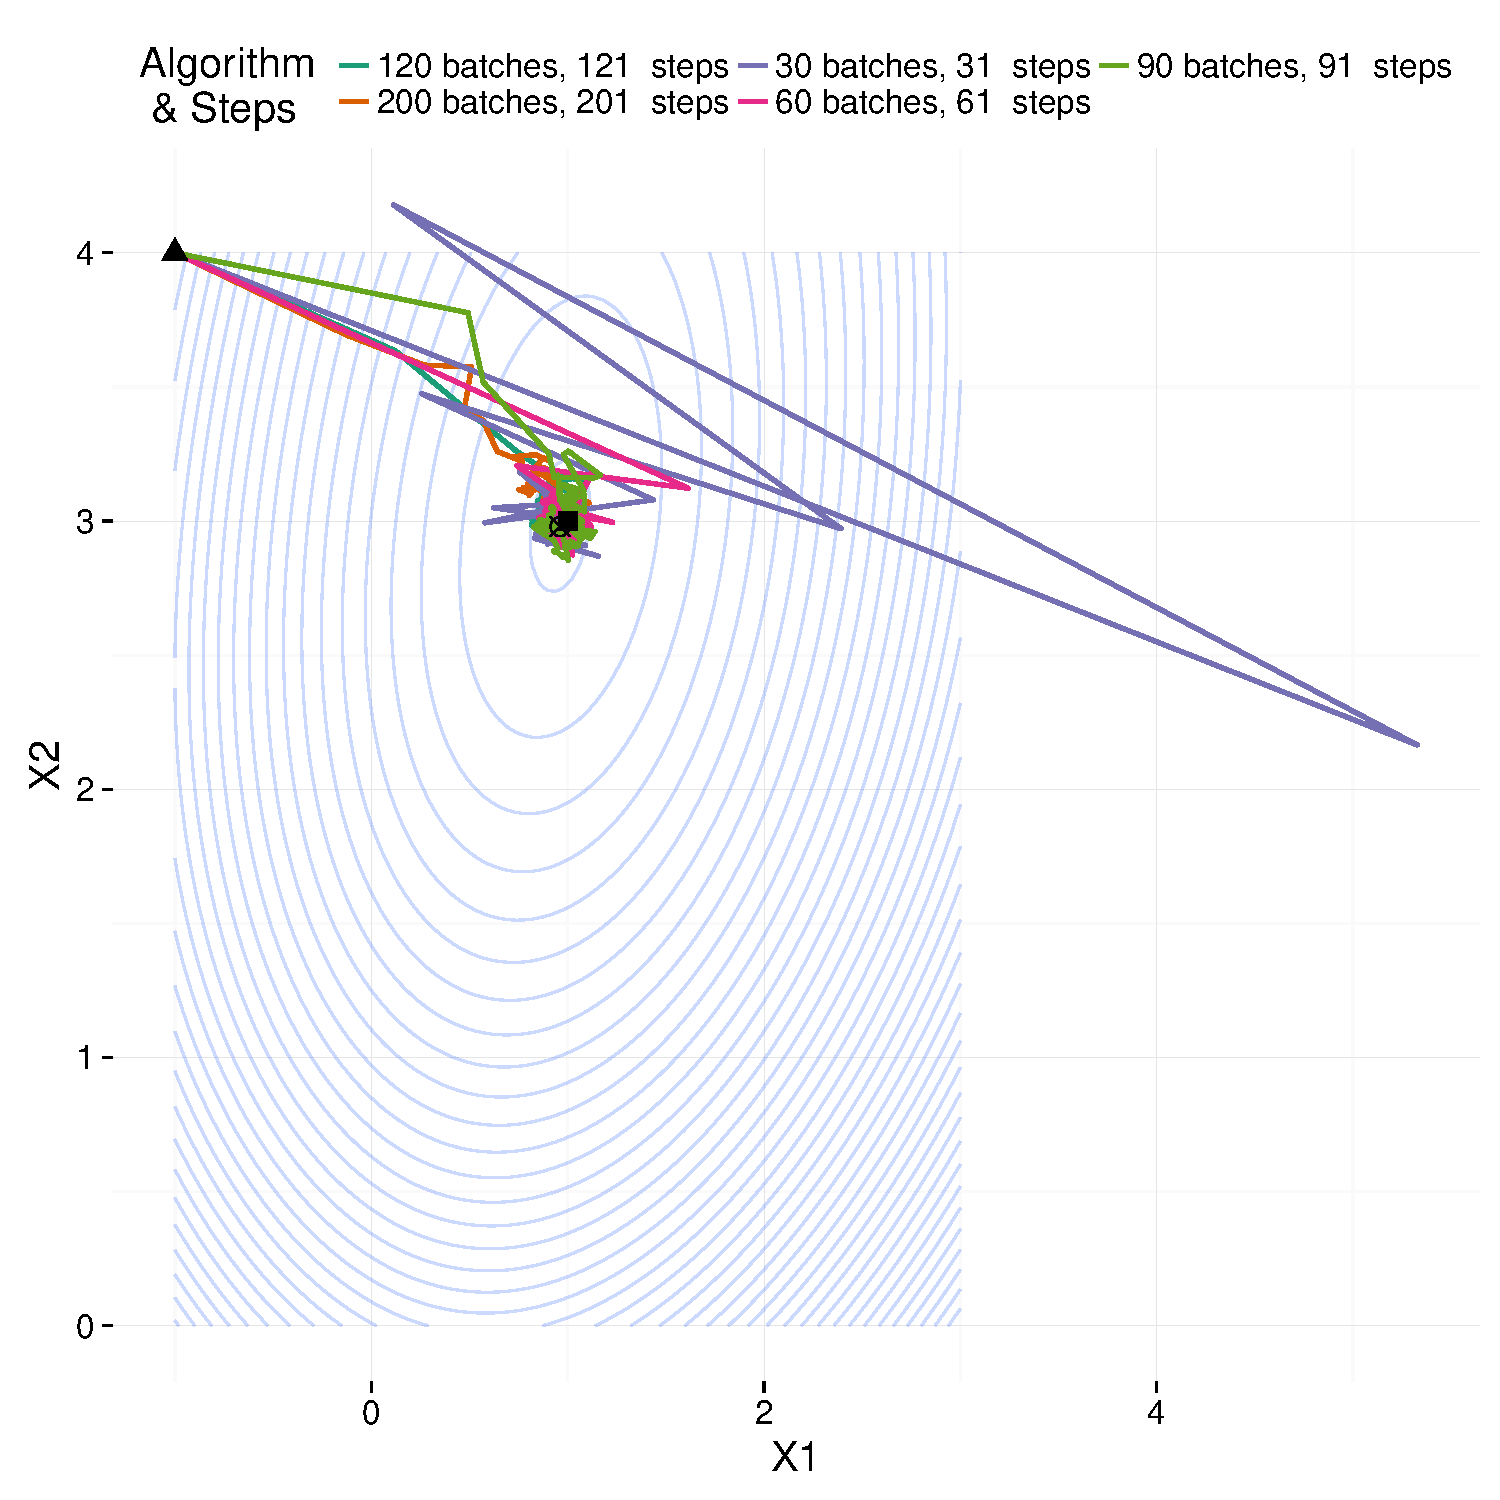
\includegraphics[width=\textwidth, height=320pt]{Obrazki/b_m1_4_iter_1_e-6_20sqrt.pdf}
      \caption{$\beta_0=(-1,4)$, liczba epok 1, warunek stopu: $\epsilon=10^{-6}$, długości kroków = $\frac{1}{20\sqrt{t}}$.}
   \end{subfigure}     
   \begin{subfigure}[h!]{0.9\textwidth}
      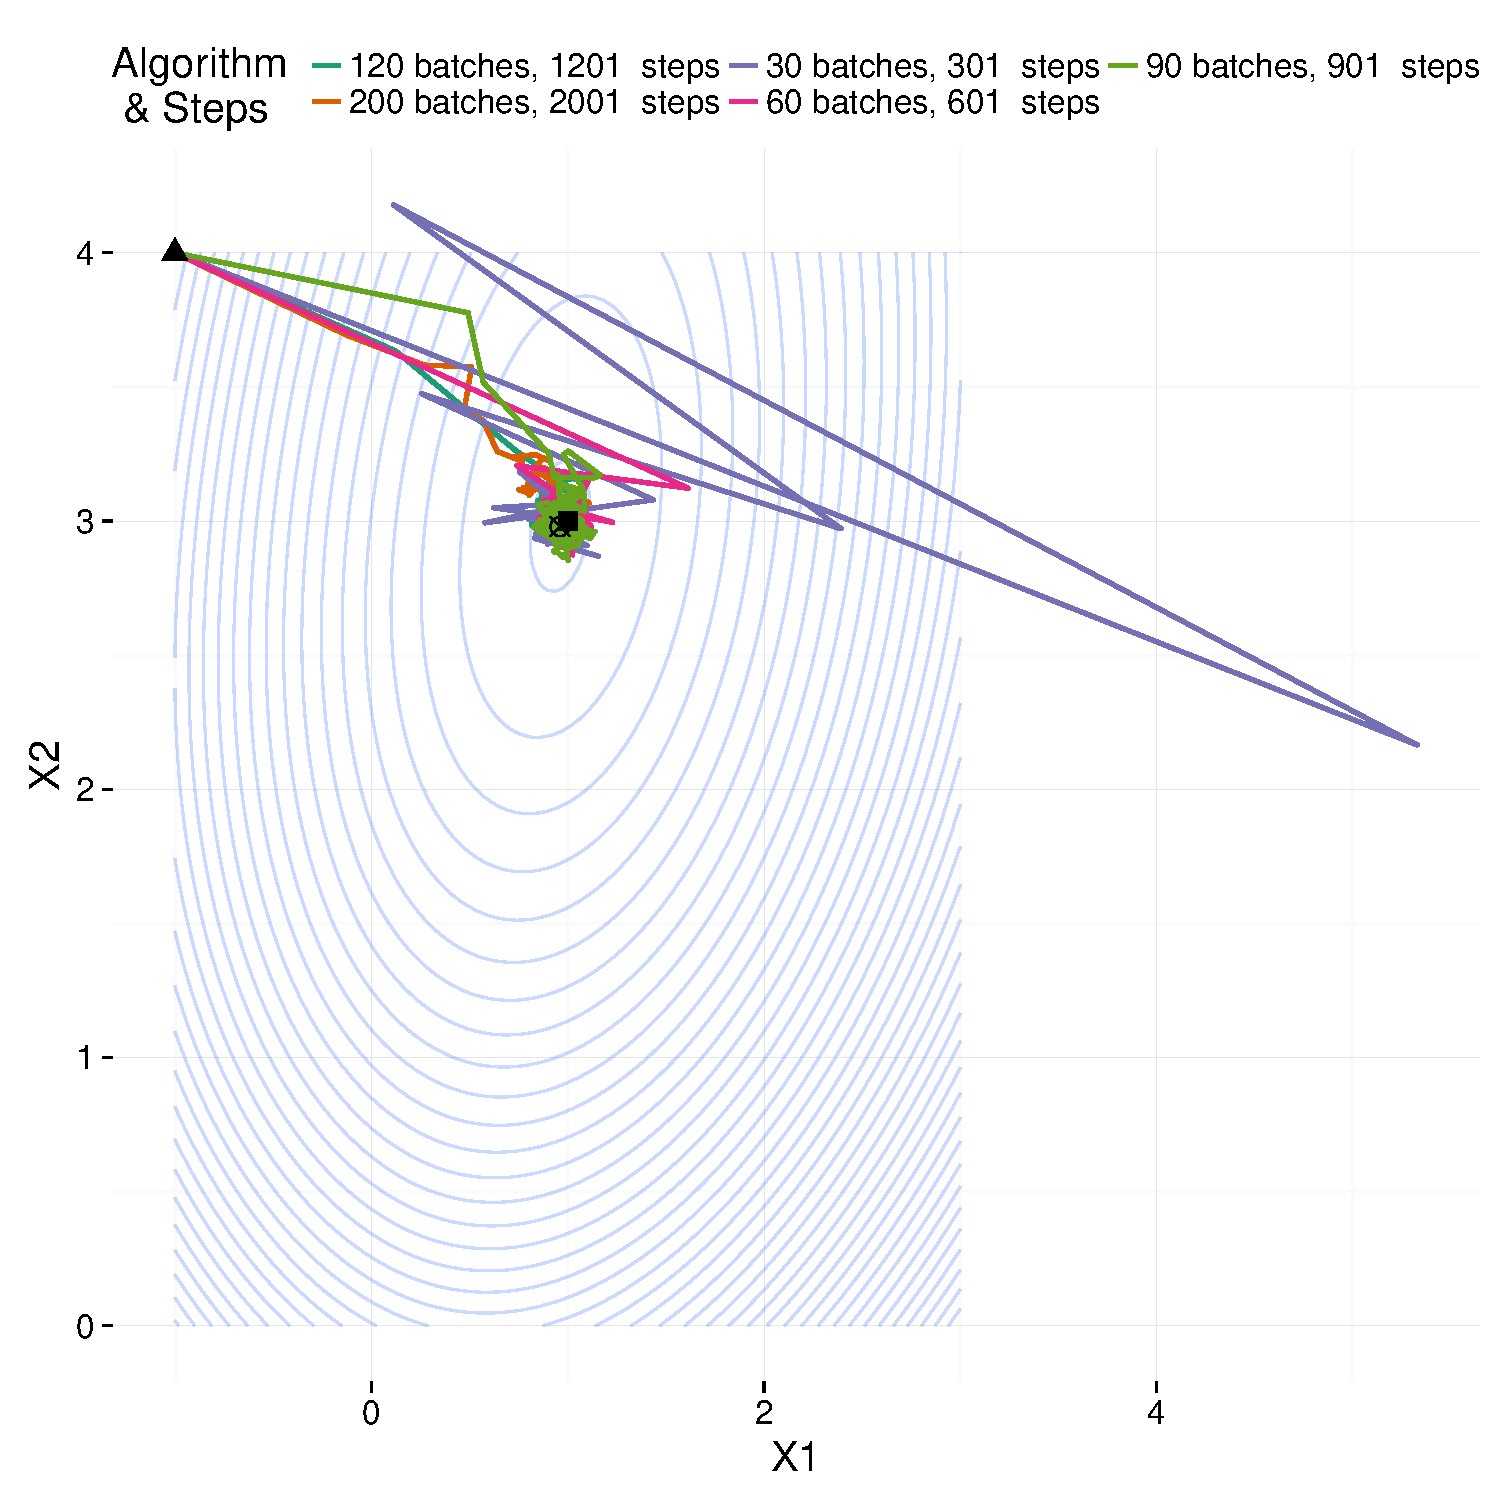
\includegraphics[width=\textwidth, height=320pt]{Obrazki/b_m1_4_iter_10_e-5_20sqrt.pdf}
            \caption{$\beta_0=(-1,4)$, liczba epok 10, warunek stopu: $\epsilon=10^{-5}$, długości kroków = $\frac{1}{20\sqrt{t}}$.}
   \end{subfigure}  
      \end{center}
  %\vspace{-10pt}
  \caption[Porównanie estymacji w modelu Coxa metodą stochastycznego spadku gradientu dla różnych podziałów zbioru początkowego na podzbiory.]{\label{rysCox4}Porównanie estymacji w modelu Coxa metodą stochastycznego spadku gradientu dla różnych podziałów zbioru początkowego na podzbiory.}
\end{figure}